\clearpage

\section{Introducción}
Un TDC (Time to Digital Converter) es un circuito electrónico capaz de medir un intervalo de tiempo y producir un valor digital. 
Fueron impulsados principalmente en el campo de la física atómica y de altas energías \cite{Altruda2023}, radares tipo LiDAR \cite{Maatta1998}, 
y aplicaciones biomédicas como tomografías por emisión de positrones (PET). Estas distintas aplicaciones normalmente utilizan  ASICs off-the-shelf para
implementarlo; sin embargo los recientes avances tecnológicos en FPGA han permitido realizar diseños
que alcanzan una precisión del orden de los pocos picosegundos, contando con la ventaja de ser flexibles y la posibilidad de integrar la aplicación
en un único dispositivo. \\

La performance de un TDC se evalúa principalmente en términos de precisión y linealidad. La precisión
es la mínima unidad que el instrumento es capaz de medir, mientras que el concepto de linealidad refiere
a la capacidad de mantener la respuesta entrada-salida de forma lineal. Son interesantes además algunos
otros aspectos como el rango de medición, tiempo muerto, consumo de energía, y frecuencia de muestreo,
sin embargo se omitirán en este trabajo.\\

En \cite{Nacho} se diseñó y fabricó 
un chip que implementa cadenas de retardo programables, donde el elemento de retardo se basa
en un inversor CMOS que mediante un registro de configuración puede añadir capacidades a su 
salida (SCI) o modificar su resistencia equivalente (CSI), como muestra la Figura \ref{fig: nacho_delay}.
Esta configuración permite la posterior ecualización de la cadena de retardos, celda a celda.
Idealmente el mínimo retardo capaz de sumarse mediante configuración es de $\tau ' = 295$pS, mientras
que experimentalmente se observó que el promedio es de $\tau ' = 340$pS. 
En este trabajo se plantea el desafío de implementar un TDC en FPGA con el fin de poder obtener 
idealmente varias muestras en el orden de las decenas de picosegundos, de modo que su resolución
permita al menos una ecualización aproximada de la cadena de retardos.

\begin{figure}[H]
      \centering
      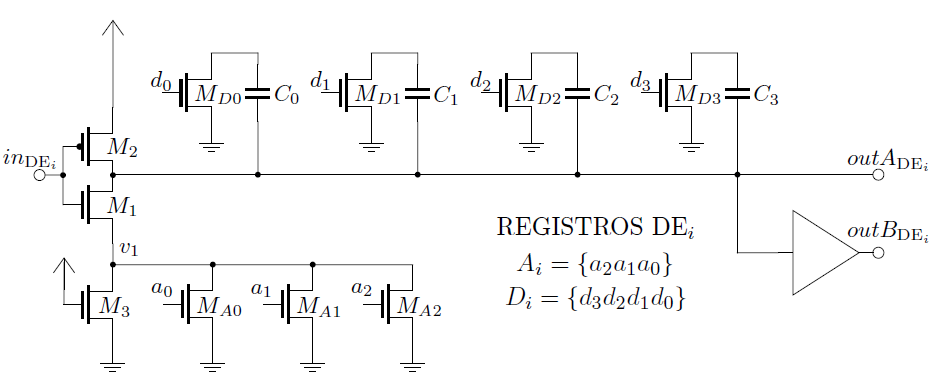
\includegraphics[width=0.75\textwidth]{imagenes/nacho_delay.png}
      \caption{Esquemático circuital del elemento de retardo.}
      \label{fig: nacho_delay}
\end{figure}

\clearpage





\section{Estado del arte}
En esta sección se explicarán algunos de los últimos avances propuestos en la bibliografía. Hasta ahora se ha hablado de
aquellos aspectos esperables en un TDC, pero es importante tener en cuenta que existen distintos paradigmas en su diseño dependiendo
de su destino: ASIC o FPGA. La libertad de colocación de componentes (placement \& routing) con 
la que se cuenta en el diseño de ASICs permite minimizar retardos indeseados que en el diseño de FPGA no tienen remedio, por tal,
esta sección será fuertemente basada en \cite{Machado} ya que propone un estudio, clasificación y análisis de las distintas 
arquitecturas bajo el paradigma de la construcción en FPGA, algo que no se había hecho hasta el momento.\\

Machado propone clasificar las distintas arquitecturas según los componentes que utiliza, de esta forma propone la taxonomía que
se muestra en la Figura \ref{fig: taxonomia}.
\begin{figure}[H]
     \centering
     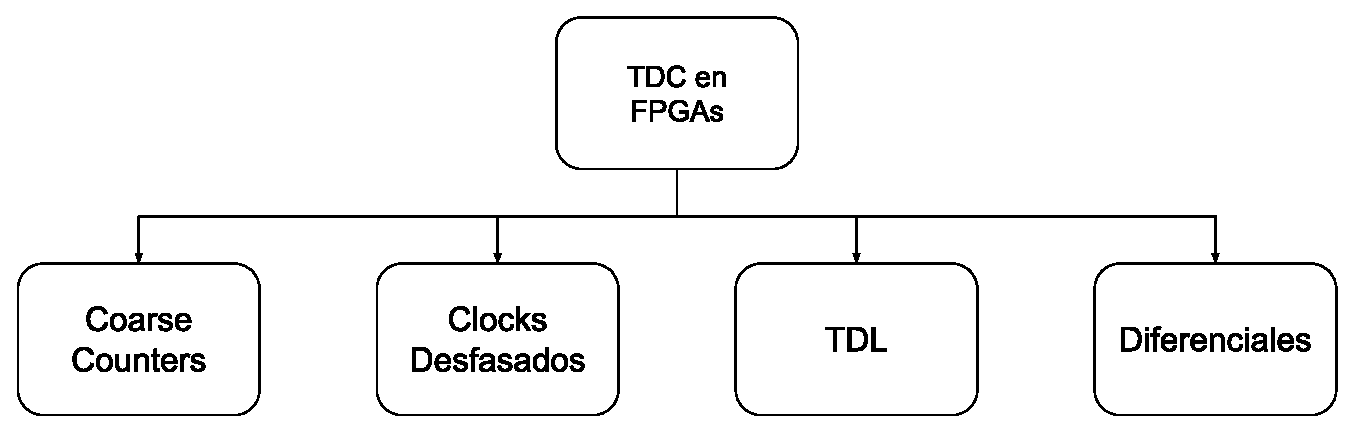
\includegraphics[width=0.75\textwidth]{imagenes/taxonomia.eps}
     \caption{Clasificación de las distintas arquitecturas.}
     \label{fig: taxonomia}
\end{figure}
Las arquitecturas de tipo \textit{Coarse Counter} (contador grueso), son aquellas que utilizan un simple contador para estimar el
ancho de pulso de una señal, según la cantidad de clocks del sistema que entran en ella; su precisión es entonces el periodo de
reloj. Las arquitecturas basadas en \textit{Clocks Desfasados} son todas aquellas que utilizan más de un clock para estimar la medición:
algunas de ellas deciden la medición a partir de saber cuál de los clocks puede observar primero la llegada del pulso, mientras que
otros utilizan elementos adicionales para la interpolación. Por otro lado está
tal vez una de las arquitecturas más utilizadas, siendo la que se aplica en este trabajo, y es aquella que utiliza \textit{Tapped Delay Lines}
(TDL: lineas de retardo registradas) para realizar la interpolación y generar la medición fina. Esto es, se ingresa el pulso 
de entrada en una cadena de elementos que introducen un retardo uniforme; al muestrear el estado de la cadena entonces
se infiere cuántos retardos la señal cruzó, con lo que se estima una medición. Dentro de esta clasificación existen distintas formas
de utilizar esta forma de interpolación, algunas arquitecturas extienden el rango de medición al combinar también un Coarse Counter, la
topología Nutt, otras utilizan varias cadenas de retardo con el fin de mejorar la precisión realizando un promedio de ellas, y otras combinan
más de una cadena y más de un clock. En cualquiera de sus formas, se clasifican según su componente principal de interpolación:
la cadena de retardos. Por último, las arquitecturas \textit{Diferenciales} se basan en medir la diferencia de retardo entre dos elementos. En
estas existen principalmente dos tipos: cadenas de retardos compuestas de dos elementos de retardo distintos, y osciladores en anillo.
Por otro lado si buscamos medir el intervalo temporal entre una señal y el clock entonces llamaremos al TDC 
\textit{síncrono}, si el intervalo puede comenzar y terminar en cualquier momento entonces lo llamaremos 
\textit{asíncrono}.\\

\subsection{Principios de la arquitectura tipo Nutt}
Las arquitecturas TDL pueden ser implementadas de distintas formas, como muestra la Figura \ref{fig: various_tdl}.
\begin{figure}[H]
     \centering
     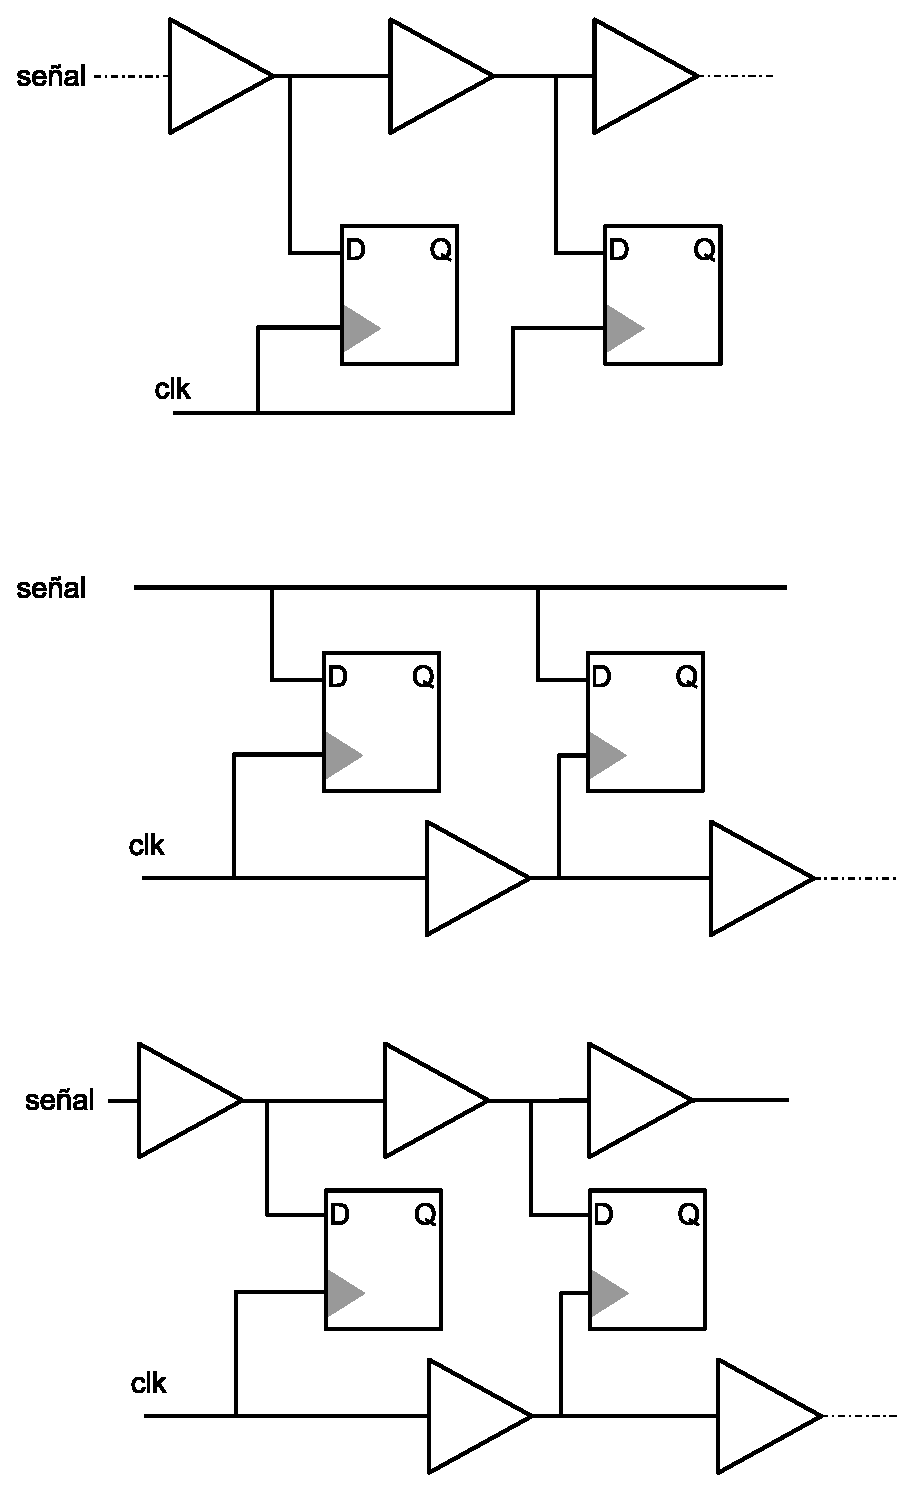
\includegraphics[width=0.75\textwidth]{imagenes/various_tdl.eps}
     \caption{Diferentes formas de aplicar el método Vernier.}
     \label{fig: various_tdl}
\end{figure}

Basicamente la señal alimenta una cadena de retardos, la cuál es registrada a cada clock. Cuando
se detecta el pulso de Start, el valor de la cadena se guarda para luego procesarlo, y componer el
resultado de parte fina, que idealmente es el espacio entre líneas rojas que muestra la Figura \ref{fig: arqui_tdl}. 
Lo mismo se realiza cuando la señal egresa de la cadena de retardos. Finalmente el resultado se compone
de una parte gruesa, y puede calcularse como
\begin{equation*}
     T_{m} = (n_{coarse}+1) \; T + \tau_{start} - \tau_{stop} 
\end{equation*}

\begin{figure}[H]
     \centering
     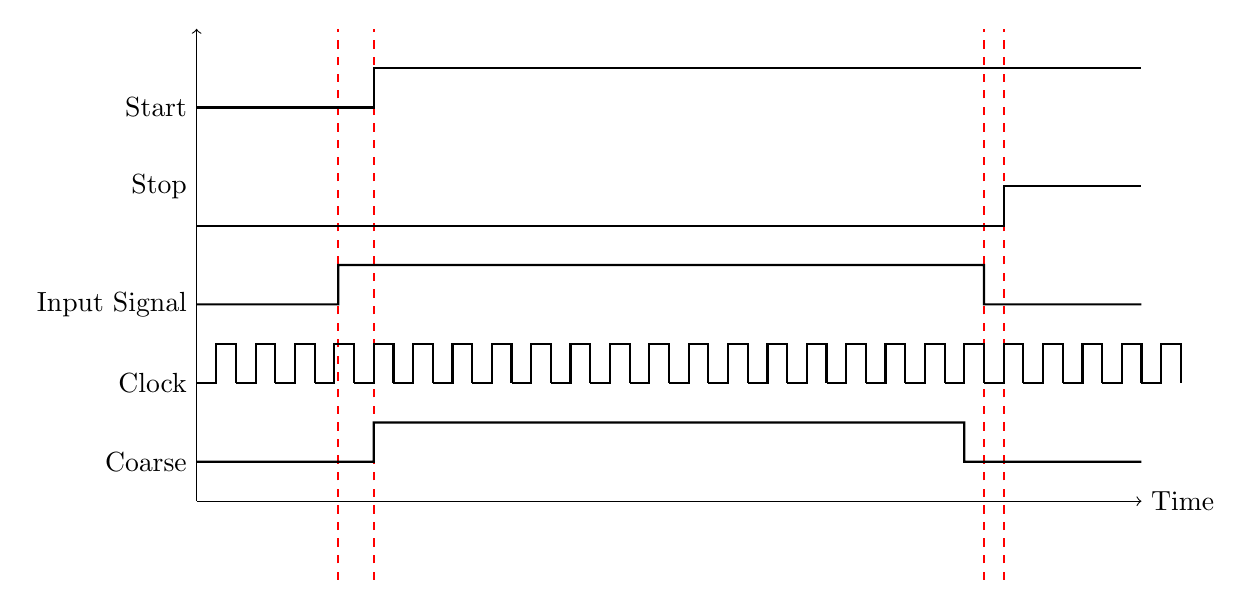
\begin{tikzpicture}
          % Define styles
          \tikzstyle{signal} = [thick]
          \tikzstyle{startstop} = [red, thick, dashed]

          % Dashed lines for START and STOP
          \draw[startstop] (1.8,-1)     -- (1.8,6);
          \draw[startstop] (2.25,-1)    -- (2.25,6);
          \draw[startstop] (10,-1)      -- (10,6);
          \draw[startstop] (10.25,-1)   -- (10.25,6);

          % Time axis
          \draw[->] (0,0) -- (12,0) node[right] {Time};

          % START signal
          \draw[signal] (0,5) -- ++(2.25, 0) -- ++(0, 0.5) -- (12,5.5);
          \node[left] at (0,5) {Start};

          % STOP signal
          \draw[signal] (0,3.5) -- (10.25,3.5) -- (10.25,4) -- (12,4);
          \node[left] at (0,4) {Stop};

          %%Input signal
          \draw[signal] (0,2.5) -- ++(1.8,0) -- ++(0,0.5) -- (10,3) -- ++(0,-0.5) -- (12,2.5);
          \node[left] at (0,2.5) {Input Signal};

          % Clock signal
          \foreach \x in {0,0.5,...,12} {
               \draw[signal] (\x, 1.5) -- ++(0.25, 0) -- ++(0, 0.5) -- ++(0.25, 0) -- ++(0,-0.5);
          }
          \node[left] at (0,1.5) {Clock};

          %%Coarse signal
          \draw[signal] (0,0.5) -- ++(2.25,0) -- ++(0,0.5) -- (9.75,1) -- ++(0,-0.5) -- (12,0.5);
          \node[left] at (0,0.5) {Coarse};


          % % Coarse Counting signal
          % \draw[signal] (2,1.5) -- (3.5,1.5) -- (3.5,1) -- (10,1) -- (10,1.5) -- (12,1.5);
          % \node[left] at (0,1.5) {Coarse Counting};

          % % Fine Counting 1 signal
          % \draw[signal] (2,0.5) -- (2.5,0.5) -- (2.5,0) -- (12,0);
          % \node[left] at (0,0.5) {Fine Counting 1};

          % % Fine Counting 2 signal
          % \draw[signal] (2,-0.5) -- (10, -0.5) -- (10, -1) -- (12, -1);
          % \node[left] at (0,-0.5) {Fine Counting 2};

          % Labels
          % \node at (6,5.2) {$T_m$};
          % \node at (6,2.8) {$T_{\text{CLK}}$};
          % \node at (6,1.7) {$T_{\text{coarse}}$};
          % \node at (2.75,0.7) {$T_{\text{fine1}}$};
          % \node at (10.5, -0.3) {$T_{\text{fine2}}$};

          % Extra line to mark the end
          \draw[<-] (0,6) -- (0, 0);

     \end{tikzpicture}
      \caption{Esquema de medición fina del pulso de entrada.}
      \label{fig: arqui_tdl}
\end{figure}

\subsection{Tests, mediciones y resultados}
Particularmente en la arquitectura TDL, la opción predilecta en la bibliografía para calibrar el instrumento es mediante 
un ``code-density test''. Esta prueba consiste en ingresar una señal decorrelacionada del reloj del sistema, de forma que 
excite todos los elementos de retardo por igual y por lo tanto ``golpee'' a cada celda por igual, generando un
histograma de hits (golpes) en función del número de celda. Si la cadena tiene
$N$ elementos, y mide un periodo de reloj $T$, y además la i-ésima celda captura $n_i$ mediciones, entonces es claro que el 
tamaño de cada retardo es
\begin{equation}
     \tau_i = n_i \; \dfrac{T}{N} \; ,
     \label{eq: tau_i}
\end{equation}
luego el retardo medio es
\begin{equation}
     \bar{\tau} = \dfrac{T}{N} \; .
     \label{eq: tau_medio}
\end{equation}
Con esto es posible calcular la DNL (Differential Non-Linearity) como
\begin{equation}
     DNL_i = \tau_i - \bar{\tau} \; ,
     \label{eq: DNL}
\end{equation}
y con esto la INL (Integral Non-Linearity) como
\begin{equation}
     INL_i = \sum_{i=0}^{N-1} {\tau_i - \bar{\tau}} \; .
     \label{eq: INL}
\end{equation}

Conociendo estas propiedades es posible generar una ``tabla de calibración''. Una vez la medición final
se realiza en el TDC, se corrige mediante una tabla pre-cargada en memoria, entregando un resultado
calibrado al instante de medición (on-line calibration \cite{Liu2015}). Se puede contemplar
una calibración exclusiva para el flanco \textit{Start} y el flanco \textit{Stop} (\cite{Khaddour2023}), y 
corregir variaciones en las condiciones PVT (\cite{Qin2017}).
Es claro que la precisión del TDC no sólo depende de un buen diseño sino que también 
se ve afectado por propiedades estadísticas, por lo tanto es posible corregir limitaciones de
hardware mediante una buena calibración.\\


%%TODO: implementar esta imágen para explicar medición
\begin{figure}[H]
      \centering
      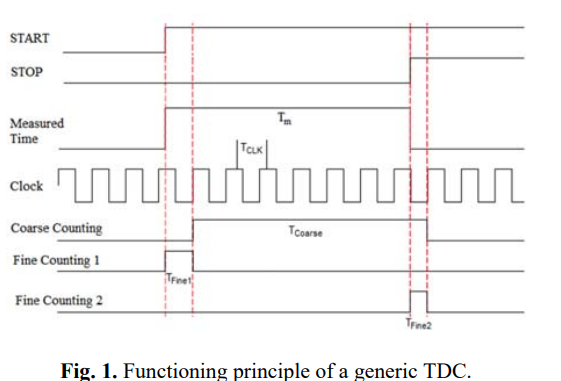
\includegraphics[width=0.75\textwidth]{imagenes/Captura de pantalla 2024-07-25 103323.png}
      \caption{Caption de prueba}
      \label{fig:prueba}
\end{figure}
\clearpage




\section{Arquitectura}

A este tipo de estructuras digitales nos gusta llamarlas \textit{ad-hoc}, ya que desde su concepción hasta su
implementación podremos ver que no se puede enmarcar dentro de una estructura típica, sino que su diseño viene estrechamente ligado
a su aplicación en particular. A simple vista puede verse que los elementos que se utilizarán, las etapas de procesamiento,
y las técnicas implementadas son poco comunes para lo que es el mundo del diseño digital. Se da a continuación 
una explicación descriptiva de cada bloque fundamental que conforma la arquitectura del \textit{TDC}.

\subsection{Tapped Delay Line}
El bloque principal de este diseño, encargado de realizar la \textit{medición fina}, es una cadena de retardos registrados.
Para implementar estos retardos existen distintas pero acotadas opciones en una implementación en FPGA. En sus
inicios la solución predilecta era utilizar multiplexores en cadena \cite{kalisz_field-programmable-gate-array-based_1997},
pero para aprovechar las ventajas propias de la estructura de una FPGA se evolucionó a utilizar
\textit{Carry4s}, posiblemente utilizado por primera vez en \cite{favi_17ps_2009}. Estos elementos
forman parte de la unidad mínima de trabajo en una FPGA, y su combinación con LUTs, Flip-Flops, y Multiplexores forman lo que 
se conoce como un \textit{SLICE}\footnote[1]{La Artix-7 cuenta con un total de 33650 slices.}. 
Los \textit{Carry4s} en su concepción fueron destinados para implementar sumadores, y tienen la ventaja de estar optimizados
para tener el mínimo retardo entre compuerta y compuerta. Además cada salida cuenta con un Flip-Flop disponible inmediatamente
luego, como se muestra en la Figura \ref{SliceYCarry}.

\begin{figure}[H]
     \centering
     \begin{subfigure}{0.45\textwidth}
           \centering
           \resizebox{\linewidth}{!}{
           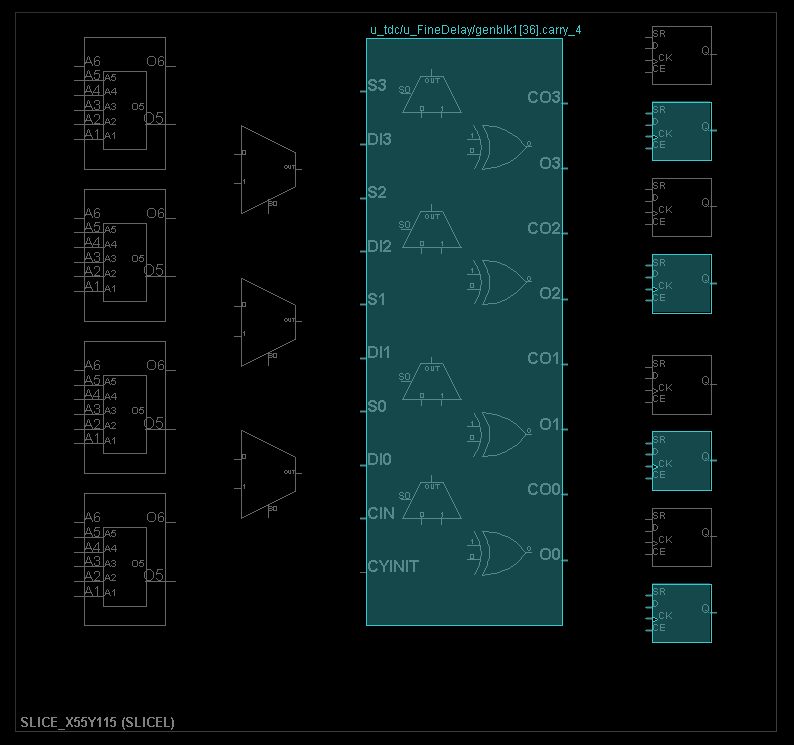
\includegraphics[]{imagenes/slice.png}
           }
           \caption{SLICE L de una Artix-7 en Vivado 2023.2}
     \end{subfigure}%
     \hspace{10pt}%
     \begin{subfigure}{0.4\textwidth}
           \centering
           \resizebox{\linewidth}{!}{
           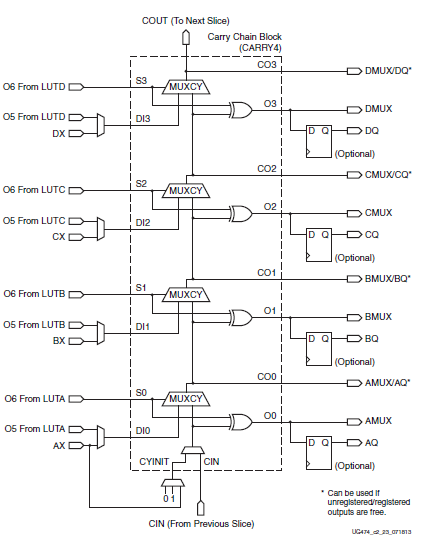
\includegraphics[]{imagenes/carry4.png}
           }
           \caption{Carry 4}
     \end{subfigure}
     \caption{Elementos disponibles dentro de una SLICE.}
     \label{SliceYCarry}
\end{figure}%

Cada Carry4 cuenta con 4 salidas que pasan por una XOR, (O0-O3) y 4 salidas que pasan por
cada MUXCY (CO0-CO3), además cuenta con un puerto \textit{CIN} con el propósito de colocarlas
en cadena y una entrada auxiliar \textit{CYINIT} desde donde ingresará el pulso externo.\\
Como la implementación aquí presentada es asíncrona precisamos capturar la señal en su flanco de entrada y de
salida de la cadena de retardos, por lo que luego de la colocación de la primer columna de Flip Flops (\textit{First} Flip Flops), 
como se ve en \ref{SliceYCarry}, se utilizan otras dos columnas de Flip Flops llamados \textit{Start} Flip Flops y \textit{Stop} 
Flip Flops. Estos se encargan de registrar la primer columna solamente cuando un flanco de subida o de bajada es detectado,
a traves de su \textit{Clock Enable}. Así se genera la estructura que se ve a continuación en la Figura \ref{fig: fine}.

\begin{figure}[H]
     \centering
     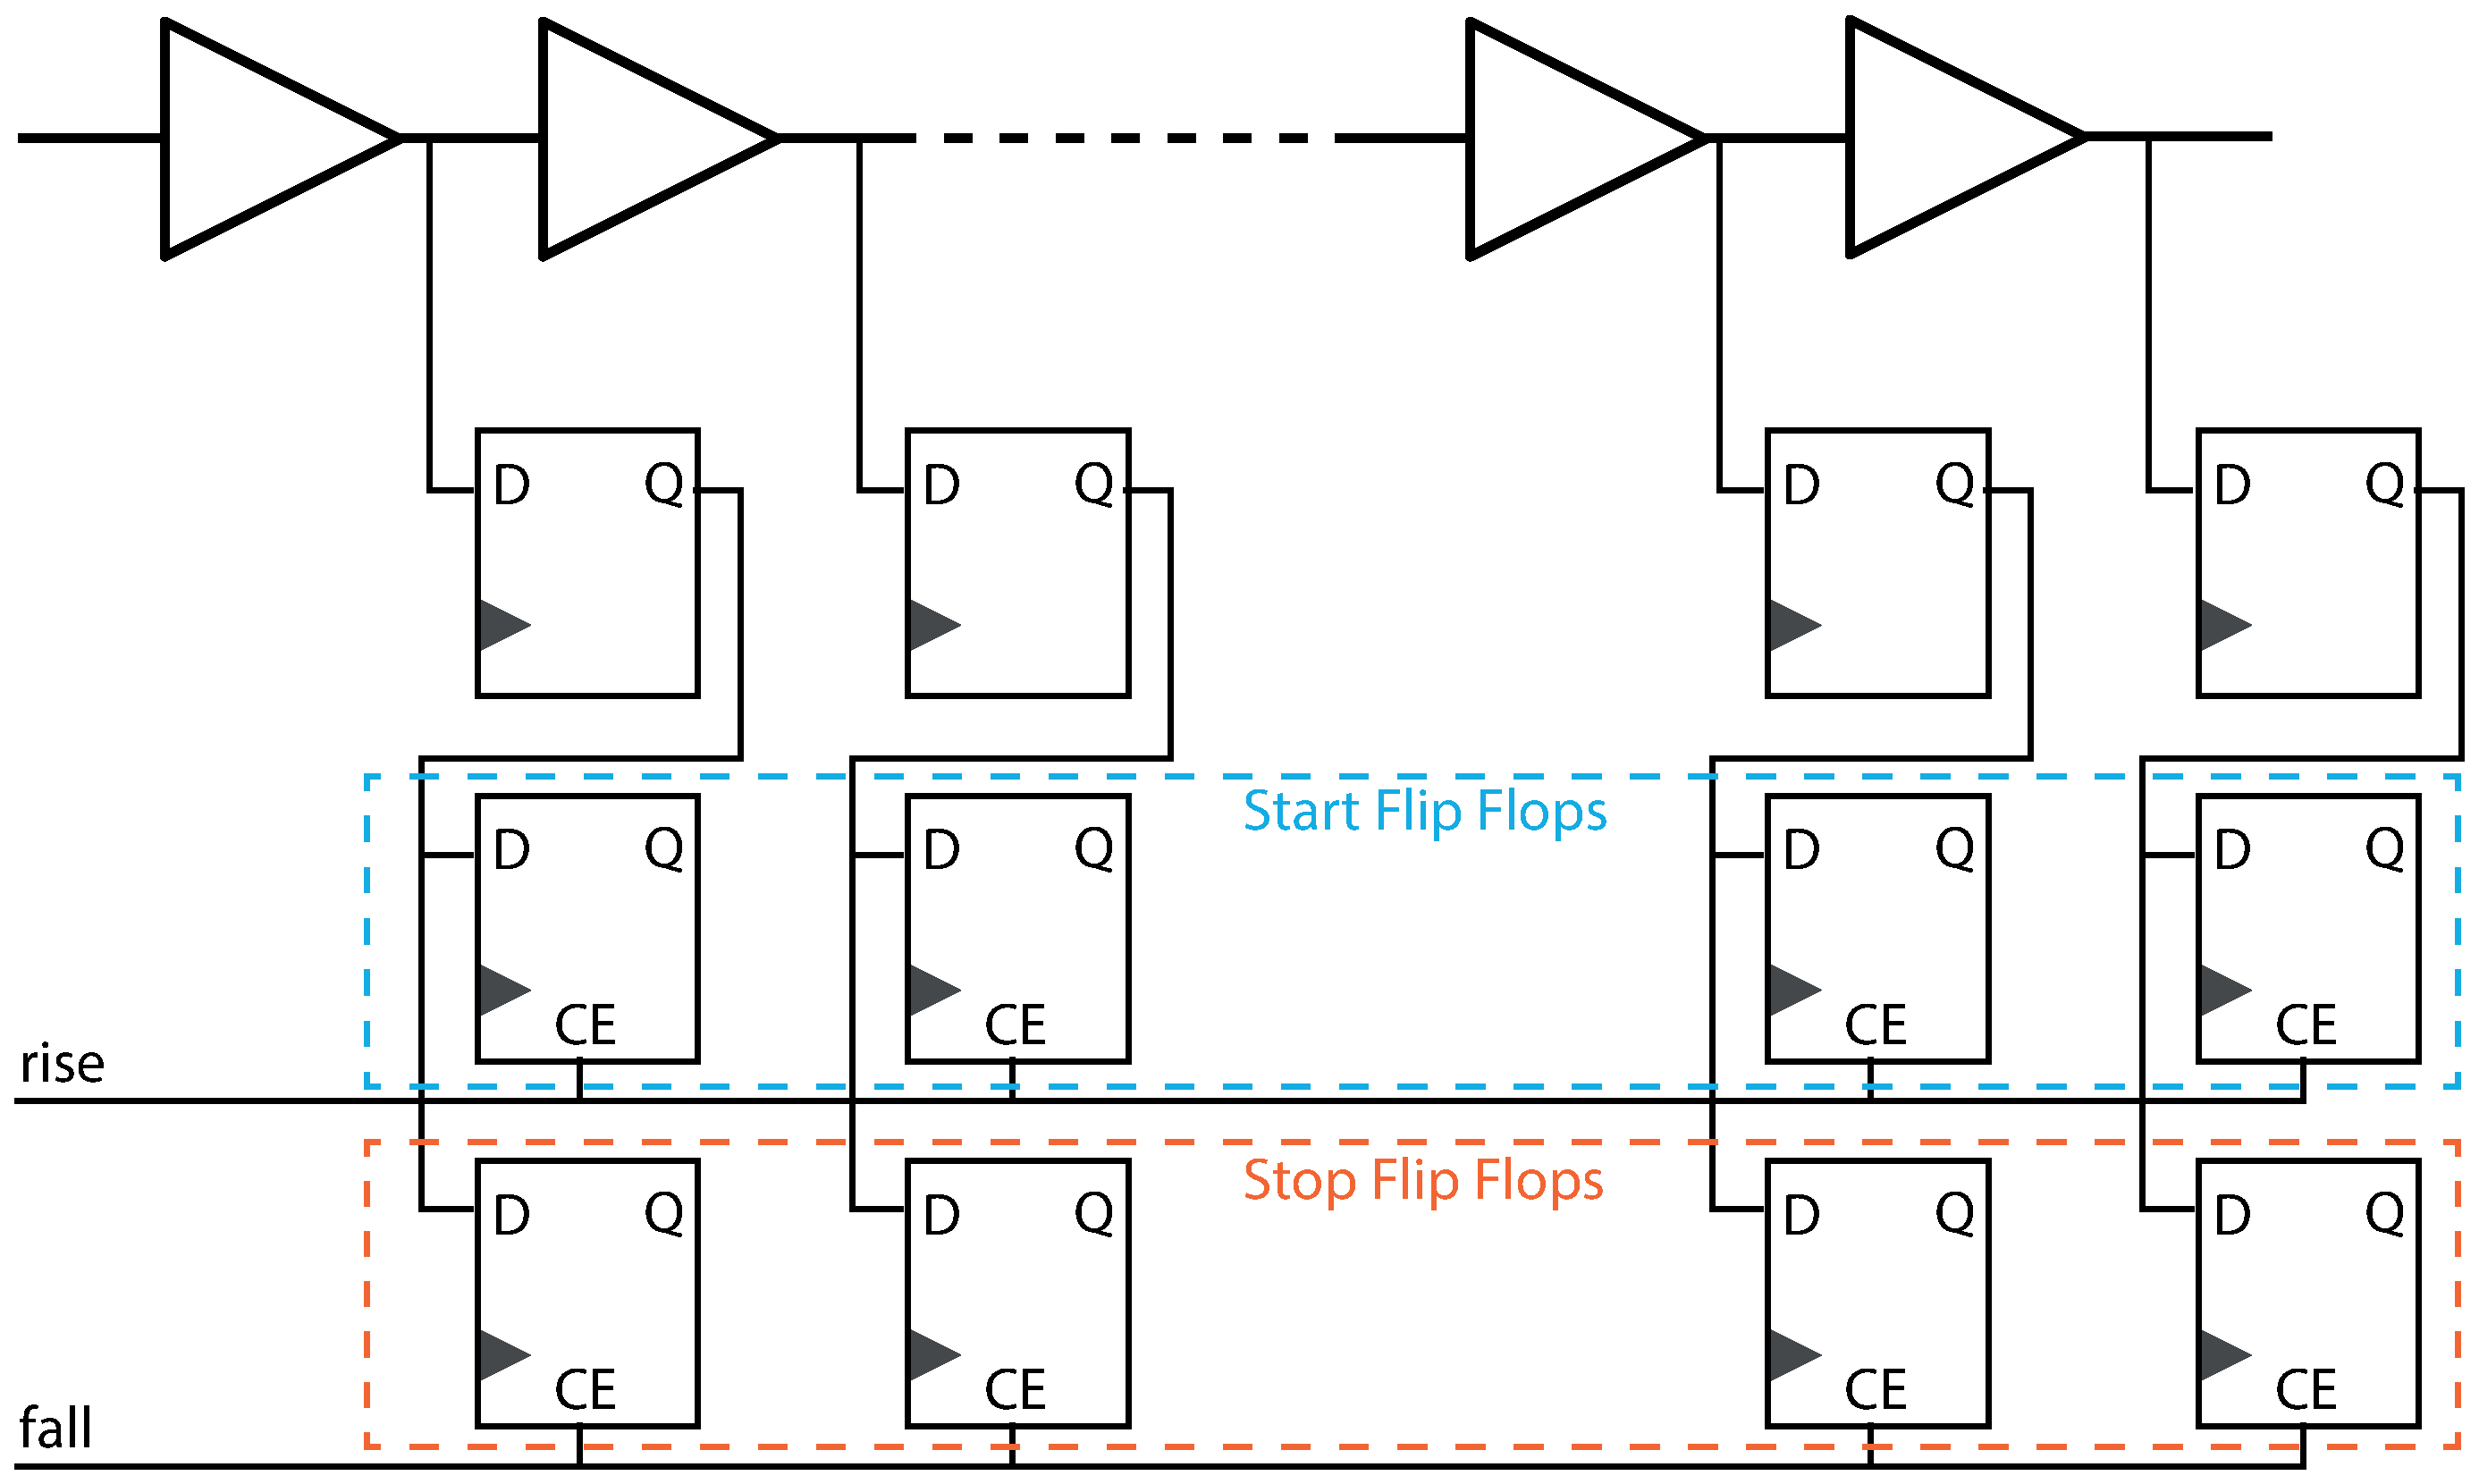
\includegraphics[width=0.7\textwidth]{imagenes/fine.eps}
     \caption{Esquema de la cadena del módulo de interpolación fina.}
     \label{fig: fine}
\end{figure}

De esta estructura surgen dos aspectos importantes:
\begin{bangenumerate}
     \item Es sabido que la transferencia de información analoga a digital puede producir metastabilidades si no se 
     realiza correctamente. La configuración de doble flip flop para registrar los elementos de retardo soluciona
     este problema introduciendo lo que se conoce como ``sincronizador''. \\
     Esto es, si el tiempo de establecimiento de la señal
     externa es menor al tiempo de establecimiento requerido por un sólo flip flop, este puede obtener
     un valor desconocido a la salida. Sin embargo introduciendo un segundo flip flop en serie, este no sufre
     de este problema, ya que para el próximo clock la señal es estable, y esta indeterminación se resuelve
     decantando hacia un estado. Además la técnica de doble registro reduce los problemas de burbujas
     en el resultado \cite{machado_novel_2018}.

     \item Una propiedad intrínseca del diseño tipo Nutt es que el tiempo del pulso a medir
     atraviese la cadena en un tiempo no menor al de un clock del sistema. Esta es una condición de diseño
     y se aprovecha en múltiples bloques, pero en particular aquí
     se puede ver que el registro de \textit{Start} y \textit{Stop} dependen de un flanco de subida o bajada para
     capturar la cadena retardos, el cuál tiene una duración de un clock.
\end{bangenumerate}

%%%%TODO: revisar lo siguiente!
Por otro lado, es importante prestar especial atención al routeo y colocación de cada elemento en el bitstream final,
pues es preponderante en la calidad de los resultados del TDC. Si los retardos introducidos por el routeo son 
uniformes para cada elemento de retardo entonces podemos asegurar que la calibración es capaz de corregir
en gran parte estos errores. Según \cite{machado_novel_2018} es importante colocar la cadena de retardos en las Slices
que quedan a continuación de los Clock Buffers, y que los flip flops sean colocados también cerca de la cadena. Esto
fue probado empíricamente y se obtuvieron mejores resultados cuando los extremos de la cadena de retardos quedaban simétricos
respecto de los clock buffers.\\
Experimentalmente se observó que cuando el extremo inferior de la cadena es lejana a los buffers, 
se pueden observar huecos en el histograma resultante, mientras que al colocarlo simétrico, este espacio
se reparte al inicio y al final de la cadena, como se ilustra en la Figura \ref{fig: problema buffer}.

\begin{figure}[H]
     \centering
     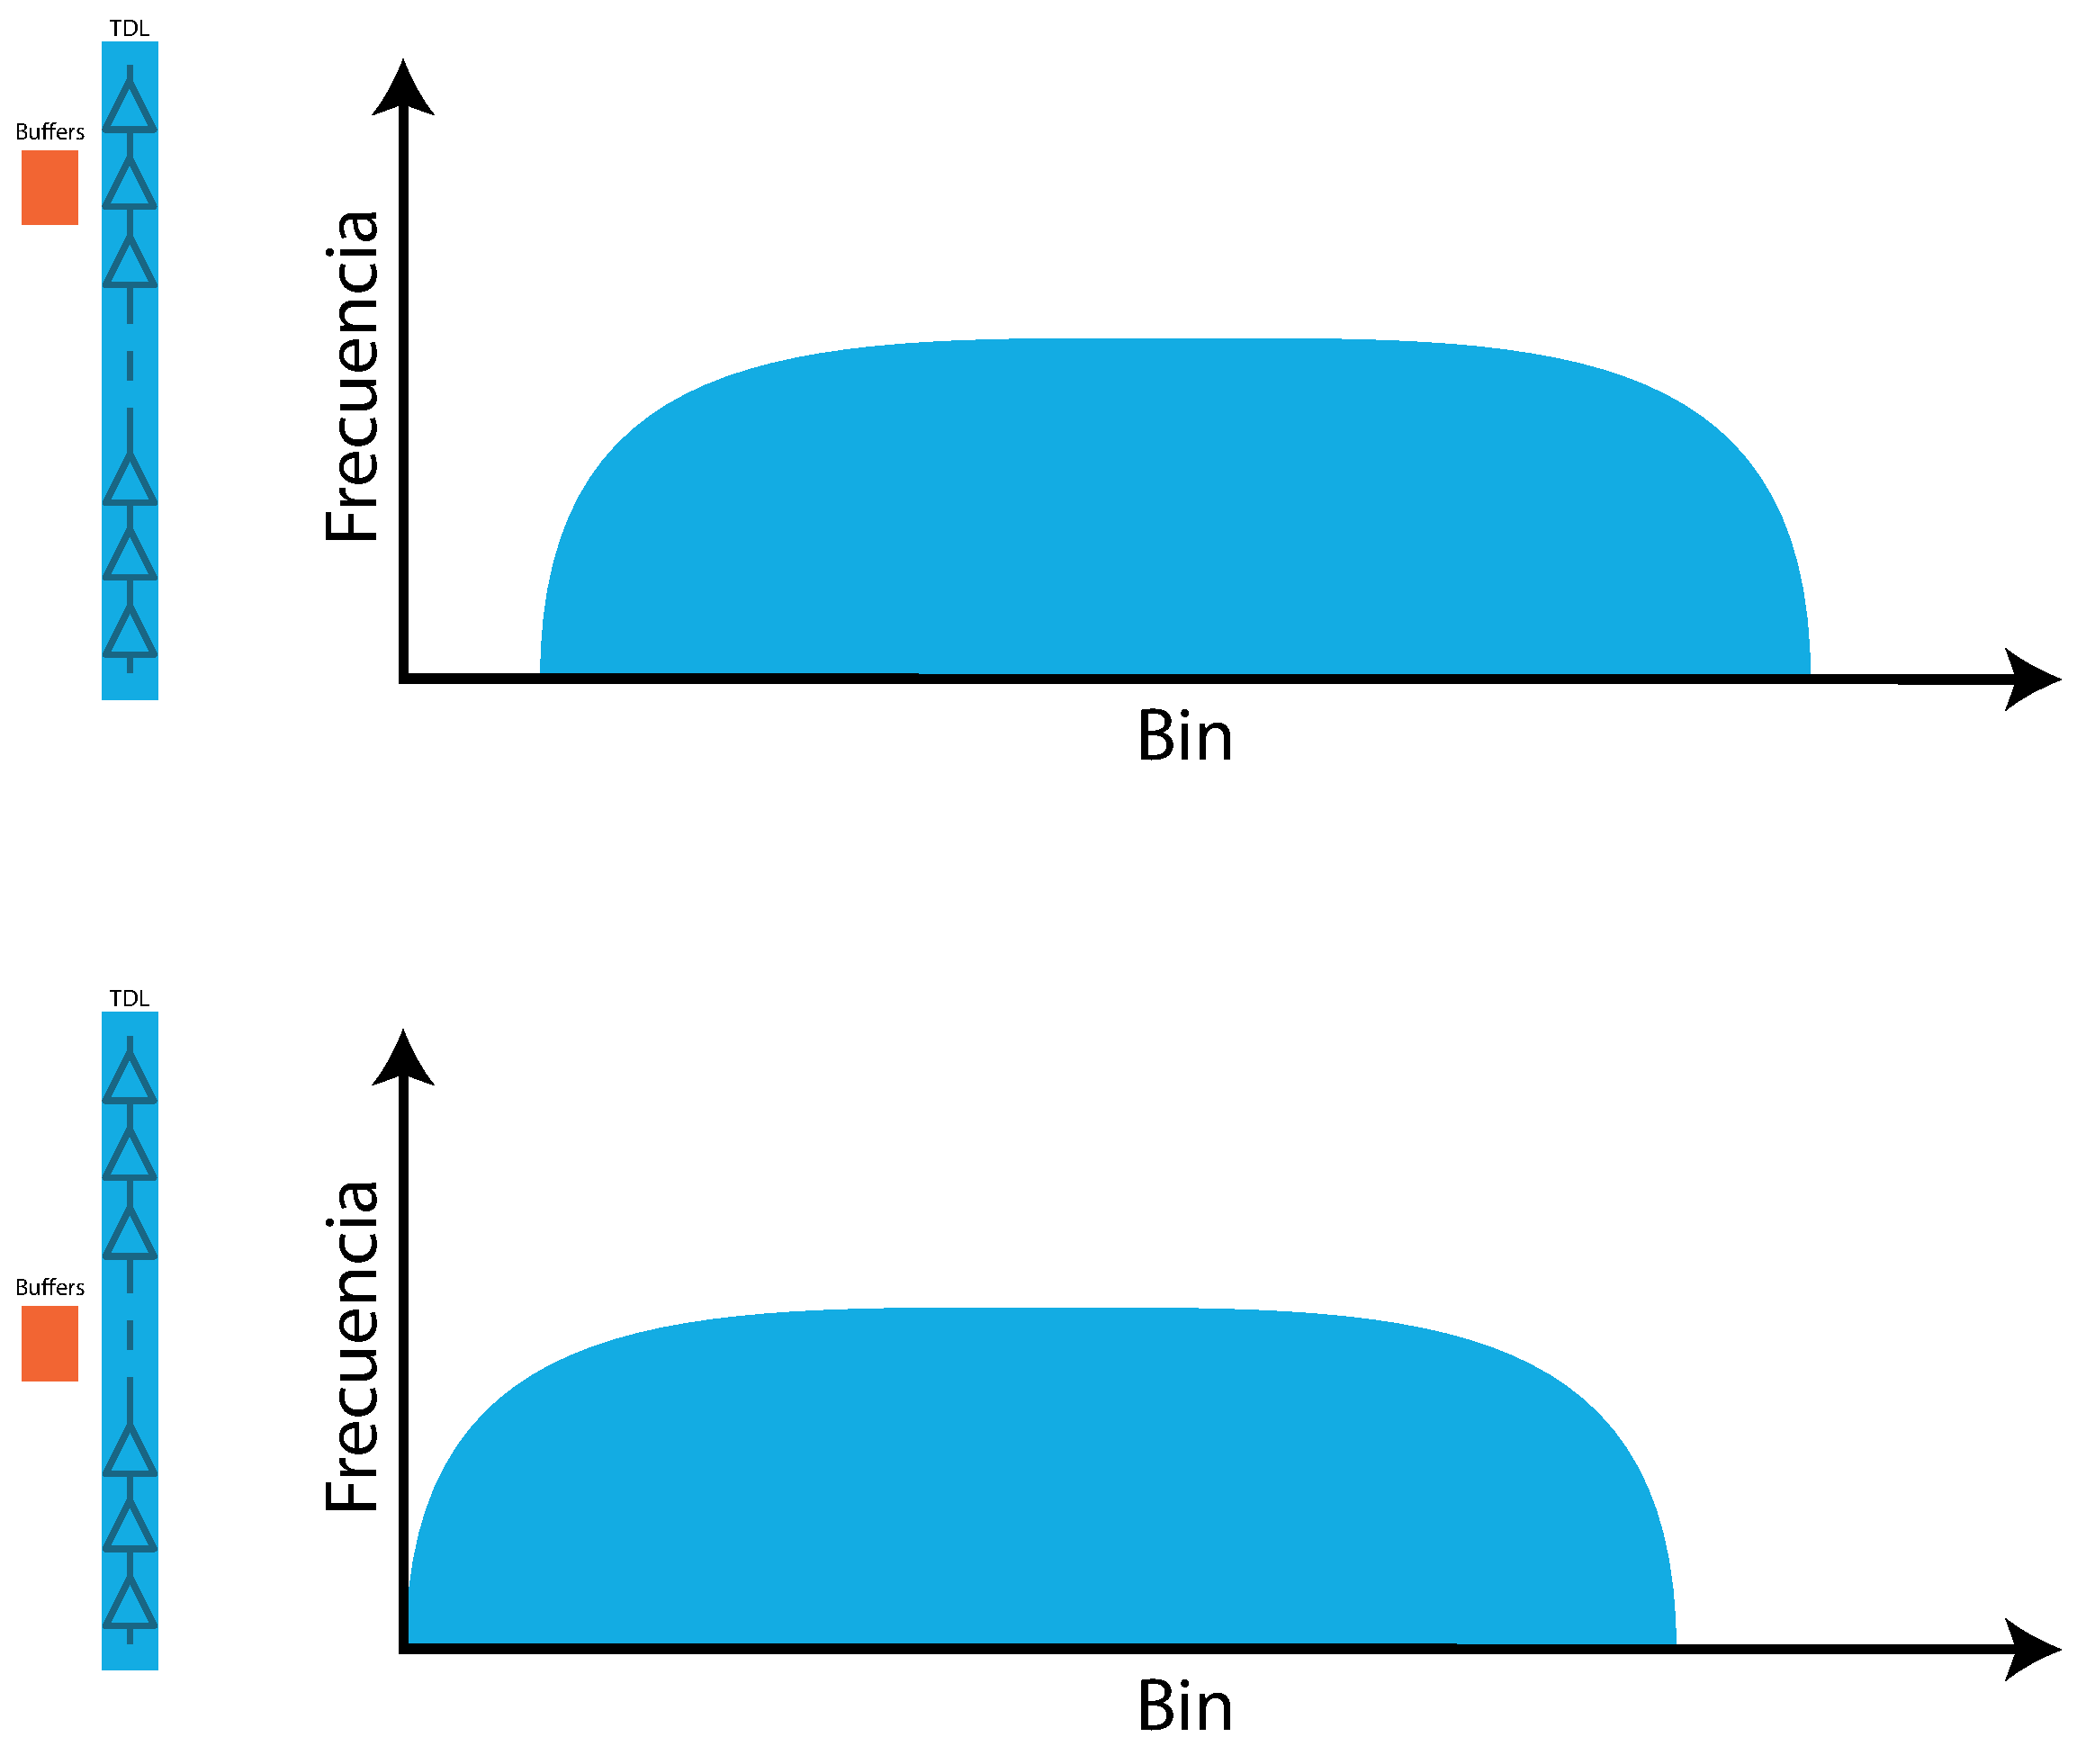
\includegraphics[width=0.75\textwidth]{imagenes/problema_buffer.eps}
     \caption{Ejemplo de histograma conseguidos al excitar el TDC con una frecuencia pseudo-aleatoria 
     modificando la posición relativa de la cadena de retardos respecto a los buffers de clock.}
     \label{fig: problema buffer}
\end{figure}

Este fenómeno tiene una explicación, y es que si la cadena de buffers mide temporalmente un clock, entonces
la posición de los buffers de clock cambia la sincronía de los Flip-Flops si no se realiza con cuidado. Los Flip-Flops
extremos son los más susceptibles a tener un mayor desfase que el resto, debido al delay de routeo. Por lo tanto al poner los buffers 
en una posición equidistante logramos compensar ese delay a ambos extremos, mientras que en el ejemplo de la Figura \ref{fig: problema buffer} 
existe un retardo mayor para el \textit{Carry4} de entrada. 

%%TODO: mencionar lo de WU-A y WU-B launcher

\subsection{Decoder}
La propagación de un pulso por la línea de retardos naturalmente genera un código unario sobre los registros. Esto
es, a medida que el flanco descendente progresa sobre la línea de retardos deja a su paso un estado alto en cada Flip-Flop de la cadena, mientra que
cuando egresa un flanco ascendente deja ceros a su paso, tal como muestra la Figura \ref{fig: tdl_flancos}.

\begin{figure}[H]
     \centering
     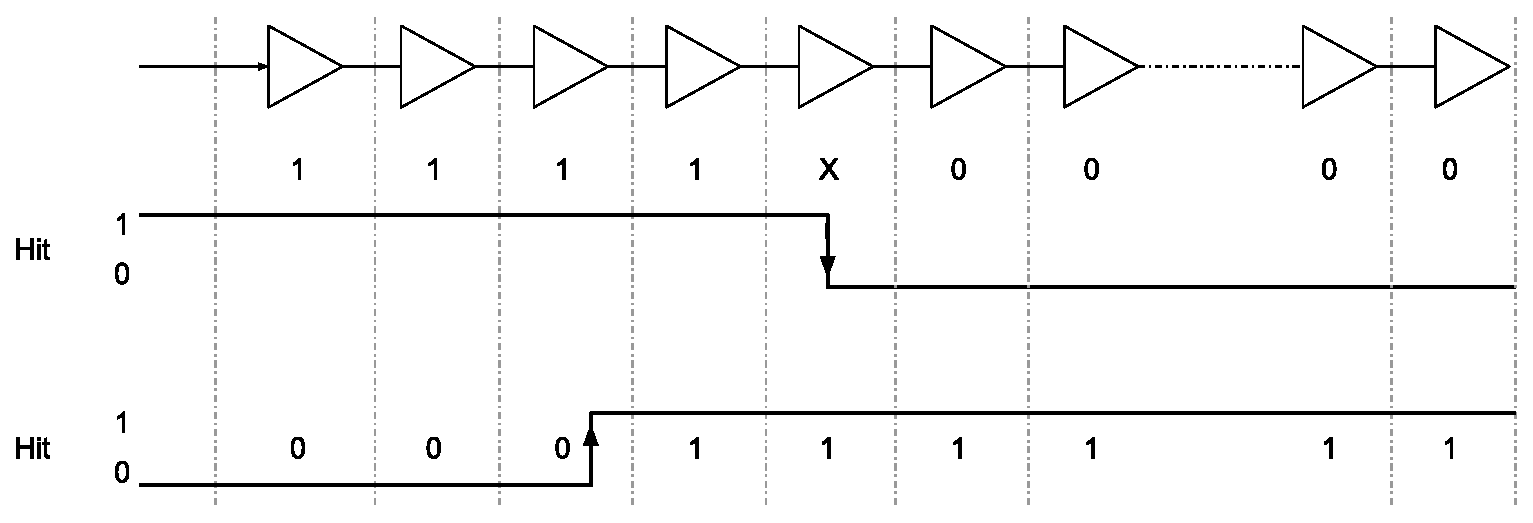
\includegraphics[width=0.75\textwidth]{imagenes/tdl_flancos.eps}
     \caption{Registro de un pulso digital en el momento que ingresa a la línea, y en el momento
     que egresa de ella.}
     \label{fig: tdl_flancos}
\end{figure}

La misión principal del decoder es traducir estos valores leídos de los registros \textit{Start} y \textit{Stop} a datos procesables. 
Aquí se presenta un gran inconveniente presente en todas las soluciones propuestas por bibliografía, pues debido a las variabilidades
propias de la arquitectura de una FPGA y de los órdenes de precisión que se pretenden es muy frecuente encontrar burbujas en los registros
resultantes, imposibilitando la utilización de decodificadores unarios convencionales. Esto significa que en los registros \textit{Start} o
\textit{Stop} se pueden encontrar registros con errores del tipo ``11..111001000...'', donde no es posible distinguir una transición de
estados clara. Según la bibliografía (\cite{Machado}) esto se debe principalmente al efecto de \textit{clock skew} cada vez más presente en los últimas tecnologías,
gracias al decrecimiento abrupto de tamaño de fabricación. Es posible que la diferencia temporal del flanco de clock (el clock skew) 
entre dos Flip Flops que registran elementos de retardo adyacentes sea mayor al tiempo de retardo de la celda a registrar, y por lo tanto 
se produce una burbuja en el registro. Esto se ejemplifica en la Figura \ref{fig: bubble}. Si el Flip-Flop número uno
captura la cadena en el momento $t_1$ y el Flip-Flop número dos lo hace un momento después en $t_2$, es posible entonces que el primero
decante su estado en un valor $0$, mientras que el segundo decante su estado en un valor $1$. La burbuja ocurre entonces si $\Delta = t_2 - t_1 \geq \tau$
siendo $\tau$ el tiempo de una celda de retardo, y $\Delta$ el clock skew.

\begin{figure}[H]
      \centering
      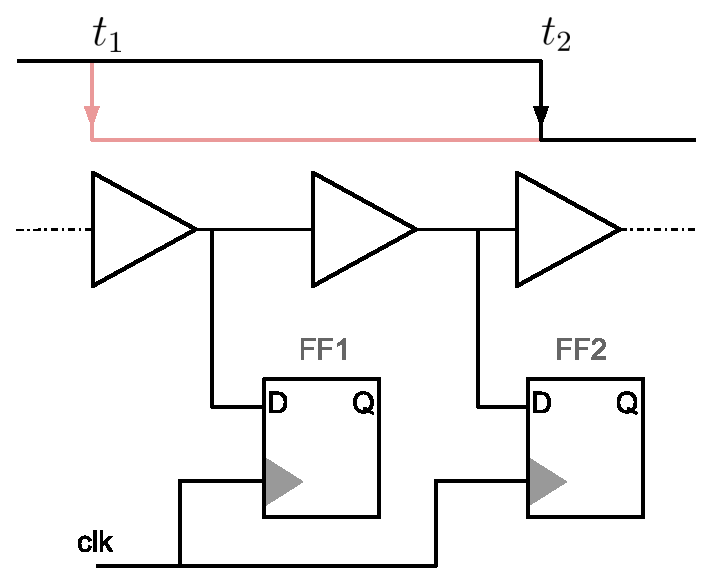
\includegraphics[width=0.55\textwidth]{imagenes/bubble.eps}
      \caption{Retardo virtual de propagación que se puede observar cuando existe \textit{clock skew} entre dos flip-flops aledaños.}
      \label{fig: bubble}
\end{figure}

Para implementar un decodificador se han propuesto distintas soluciones, en este sección resumiremos las ideas más usadas:
\begin{bangenumerate}
     \item \textbf{Contador de unos (ones counter):} se propuso como una solución en el diseño de ADCs, y luego en \cite{wang_39-ps_2017} se utiliza por primera vez
     para el diseño de un TDC. La implementación consiste básicamente en contar la cantidad de estados altos en el registro para definir la posición aproximada del flanco. 
     Si se puede asegurar que la cantidad de burbujas es despreciable entonces la respuesta del decodificador se acerca a la real. Esto es beneficioso porque 
     se prescinde del ordenamiento de un registro, es decir la entrada ``111100'' se decodificaría en la misma respuesta que la entrada ``111010'', por lo tanto
     tiene la habilidad natural de corregir errores de burbuja.

     \item \textbf{Buscador de flancos:} Consiste en realizar un circuito combinacional que busque secuencialmente (look-for) transiciones de estados del tipo ``0-1'' o ``1-0'' en el
     registro de entrada y devuelva la posición de este dentro la cadena, e.g para un registro ``0001111111'' el decoder debe devolver tres, ya que es la
     posición donde se detecta la transición. Para eliminar el problema de burbujas se recurre a aumentar el tamaño de la secuencia buscada,
     es decir si se tiene un registro con burbujas del tipo ``0001001111'' podemos buscar la secuencia ``0001'' de forma que únicamente la primer transición es detectada
     y la burbuja se ignora (\cite{Wu2010}). Rápidamente se hace evidente que a medida que el tamaño del filtro incrementa es capaz de corregir burbujas
     de mayor tamaño, a costa de descartar una mayor cantidad de muestras al principio y final de la cadena.
     
     
     \item \textbf{Realineamiento de taps:} Una vez detectados los lugares del registro donde se producen burbujas, se intercambia la posición de salida
     de estos flip-flops con el de uno cercano (\cite{Liu2015}), luego se utiliza un decoder del tipo ``buscador de flancos''. Para su implementación primero
     se debe hacer un ``code-density test'' que nos permita conocer cuáles son los bines de tamaño cero (burbujas), para luego realizar el reordenamiento de taps. Esta
     implementación depende fuertemente de las condiciones PVT\footnote{Proceso, voltaje y temperatura.} en las que se utiliza la FPGA.
\end{bangenumerate}

\subsection{Medición gruesa y Árbitro}
Una de las ventajas de la implementación tipo Nutt es que nos permite mantener un buen rango de medición sin perder precisión. Esto se logra separando la implementación en dos tareas, 
la medición gruesa y la medición fina, para esto se utiliza un contador grueso (coarse counter) con el que se mide la cantidad de periodos de clocks que tarda la señal en atravesar la cadena.
Aunque esta propuesta parece sencilla precisa de una sincronización previo al procesamiento del resultado, ya que si la señal externa entra en sincronía con el clock del sistema es posible que
el contador cuente o no un periodo de reloj menos, perdiendo una precisión de un periodo completo. En \cite{machado_novel_2018} se propone la utilización de más de un contador grueso como árbitros
para decidir el resultado final del cálculo, el desarrollo es el siguiente:\\

Se implementaron tres contadores gruesos, cada uno alimentado por un clock derivado del clock del sistema y ligeramente desfasado, como se muestra
en la Figura \ref{fig: arbitro}.
\begin{figure}[H]
     \centering
     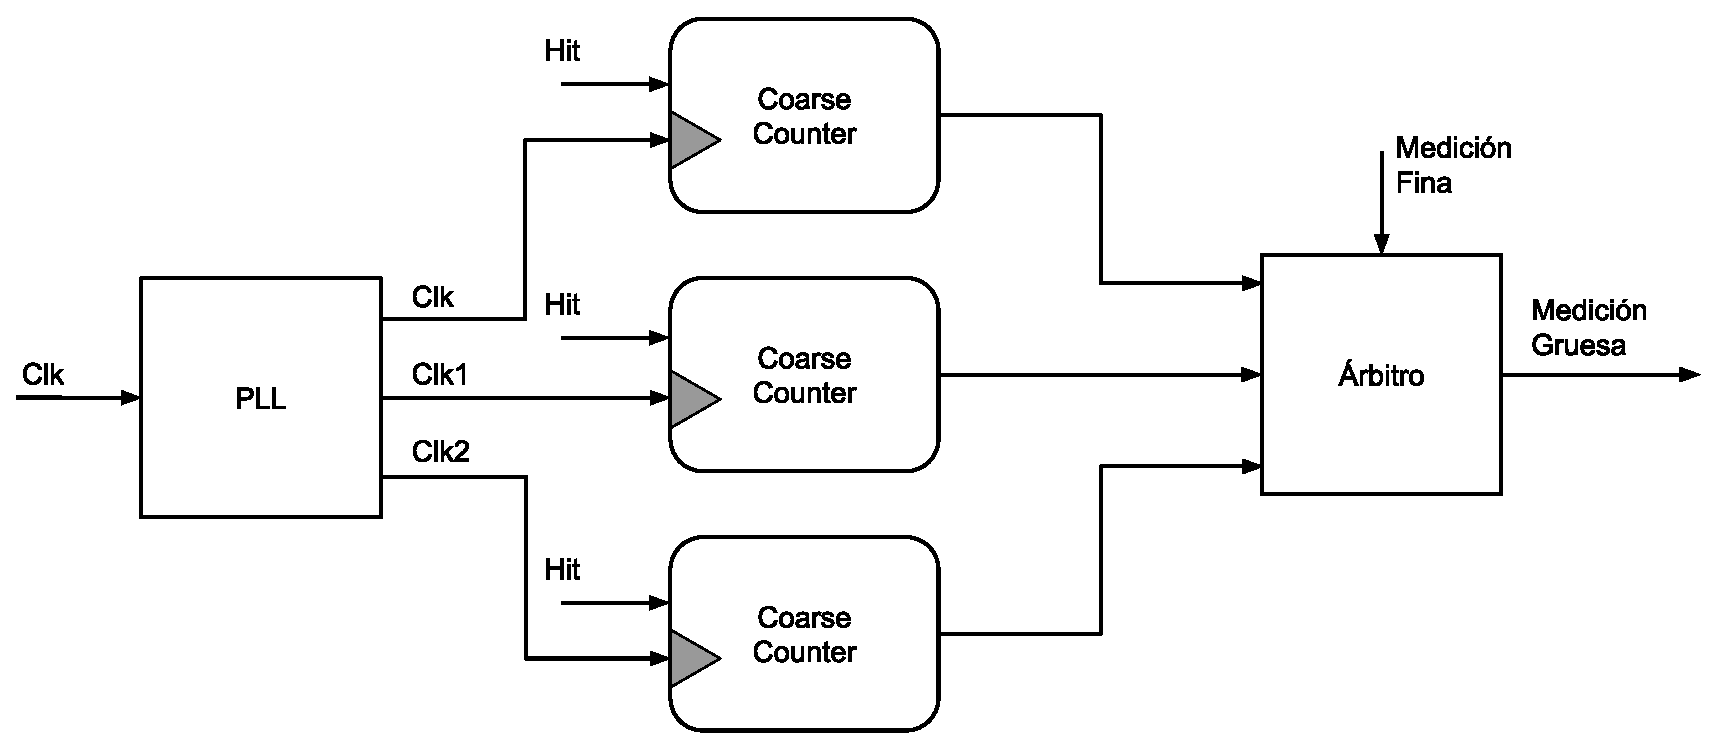
\includegraphics[width=0.75\textwidth]{imagenes/arbiter.eps}
     \caption{Arbitro implementado.}
     \label{fig: arbitro}
\end{figure}

Estos tres clocks inducen cuatro casos a diferenciar, estos se plantearan
para el flanco de entrada pero
puede hacerse de la misma forma para el flanco de salida.\\
El caso base es suponer que el pulso llega antes del flanco de subida de todos los clocks,
como muestra el Caso I de la Figura \ref{fig: casos_arbitro}, o también llegar entre cada par de flancos como muestran los Casos II, III y IV.
Para el primer caso, la línea de retardos captura la señal al inicio de la cadena pues el clock ocurre cerca de la llegada del pulso, sin embargo
para el resto de casos donde el flanco de clock ya ocurrió es necesario esperar un periodo al próximo flanco de clock, en consecuencia se captura el flanco de entrada
al borde de saturar la cadena de retardos, como muestra la Figura \ref{fig: finos_casos_start}.\\

\begin{figure}[H]
     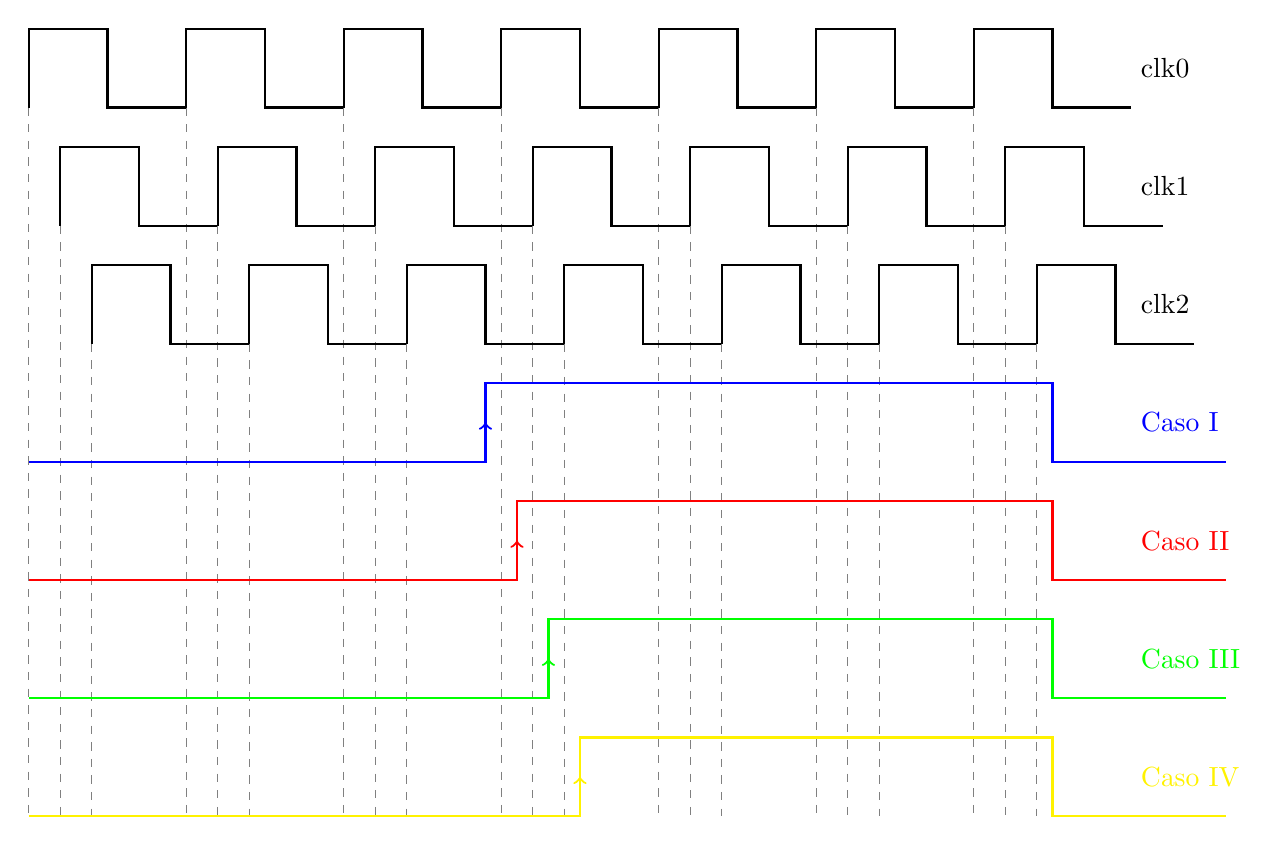
\begin{tikzpicture}
          % Define parameters
          \def\amplitude{1}       % Amplitude of the square waves
          \def\period{2}          % Period of the square waves
          \def\phaseShift{0.2}    % Phase shift for each wave (in terms of period fraction)
          \def\yShift{1.5}        % Vertical shift for each wave
          \def\stepLength{8}      % Total length for the step signal (4 periods)
          \def\stepPhaseShift{0.2}% Phase shift for step signals
      
          \def\Longtotal{15}

          % Draw clk0
          \foreach \x in {0, 2, 4, 6, 8, 10, 12} {
              \draw[thick, black] (\x, 0) -- ++(0, \amplitude) -- ++(1, 0) -- ++(0, -\amplitude) -- ++(1, 0);
              \draw[dashed, gray] (\x, 0) -- (\x, -6*\yShift cm);
          }
          \node[black, right] at (14, 0.5*\amplitude) {clk0};
      
          % Draw clk1
          \foreach \x in {0, 2, 4, 6, 8, 10, 12} {
              \draw[thick, black, yshift=-\yShift cm] (\x + \phaseShift * \period, 0) -- ++(0, \amplitude) -- ++(1, 0) -- ++(0, -\amplitude) -- ++(1, 0);
              \draw[dashed, gray] (\x + \phaseShift * \period, -\yShift cm) -- (\x + \phaseShift * \period, -6*\yShift cm);
          }
          \node[black, right] at (14, 0.5*\amplitude - \yShift) {clk1};
      
          % Draw clk2
          \foreach \x in {0, 2, 4, 6, 8, 10, 12} {
              \draw[thick, black, yshift=-2*\yShift cm] (\x + 2*\phaseShift * \period, 0) -- ++(0, \amplitude) -- ++(1, 0) -- ++(0, -\amplitude) -- ++(1, 0);
              \draw[dashed, gray] (\x + 2*\phaseShift * \period, -2*\yShift cm) -- (\x + 2*\phaseShift * \period, -6*\yShift cm);
          }
          \node[black, right] at (14, 0.5*\amplitude - 2*\yShift) {clk2};
      
          % Draw step signal cases
      
          % Case 1: Rising edge 0.2 to the left of the third clk0 rising edge
          \foreach \x in {6 - 0.2} {
              \draw[thick, blue, yshift=-3*\yShift cm] (0, 0) -- (\x, 0) -- ++(0, \amplitude) -- ++(\stepLength-\period + 1.2, 0) -- ++(0, -\amplitude) -- ++(\Longtotal - \x - \stepLength + \period - 0.6, 0);
              \draw[->, thick, blue] (\x, -3*\yShift cm) -- ++(0, 1/2*\amplitude);
          }
          \node[blue, right] at (14, 0.5*\amplitude - 3*\yShift) {Caso I};
      
          % Case 2: Rising edge 0.2 to the right of the third clk0 rising edge
          \foreach \x in {6 + 0.2} {
              \draw[thick, red, yshift=-4*\yShift cm] (0, 0) -- (\x, 0) -- ++(0, \amplitude) -- ++(\stepLength - \period + 1 - 0.2, 0) -- ++(0, -\amplitude) -- ++(\Longtotal - \x - \stepLength + \period - 1, 0);
              \draw[->, thick, red] (\x, -4*\yShift cm) -- ++(0, 1/2*\amplitude);
          }
          \node[red, right] at (14, 0.5*\amplitude - 4*\yShift) {Caso II};
      
          % Case 3: Rising edge 0.6 to the right of the third clk0 rising edge
          \foreach \x in {6 + 0.6} {
              \draw[thick, green, yshift=-5*\yShift cm] (0, 0) -- (\x, 0) -- ++(0, \amplitude) -- ++(\stepLength - \period +1 -0.6, 0) -- ++(0, -\amplitude) -- ++(\Longtotal - \x - \stepLength + \period - 1.4, 0);
              \draw[->, thick, green] (\x, -5*\yShift cm) -- ++(0, \amplitude/2);
          }
          \node[green, right] at (14, 0.5*\amplitude - 5*\yShift) {Caso III};
      
          % Case 4: Rising edge 1 to the right of the third clk0 rising edge
          \foreach \x in {6 + 1} {
              \draw[thick, yellow, yshift=-6*\yShift cm] (0, 0) -- (\x, 0) -- ++(0, \amplitude) -- ++(\stepLength - \period +1 -1, 0) -- ++(0, -\amplitude) -- ++(\Longtotal - \x - \stepLength + \period - 1.8, 0);
              \draw[->, thick, yellow] (\x, -6*\yShift cm) -- ++(0, \amplitude/2);
          }
          \node[yellow, right] at (14, 0.5*\amplitude - 6*\yShift) {Caso IV};
     \end{tikzpicture}
     \caption{Todos los casos posibles de arbitraje para el flanco Start}
     \label{fig: casos_arbitro}
\end{figure}

\begin{figure}[H]
     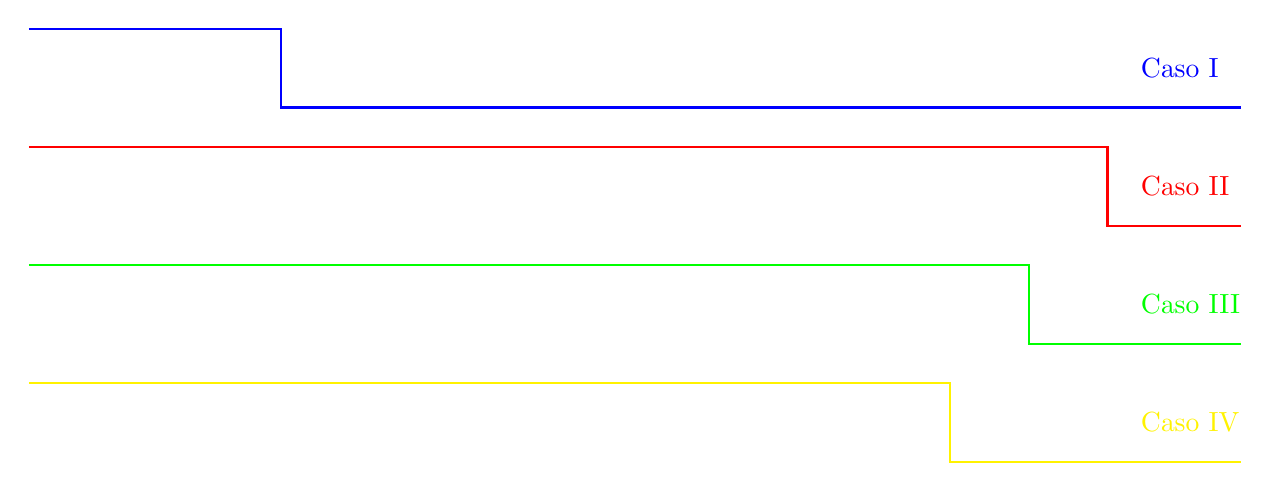
\begin{tikzpicture}
          % Define parameters
          \def\amplitude{1}       % Amplitude of the square waves
          \def\period{2}          % Period of the square waves
          \def\phaseShift{0.2}    % Phase shift for each wave (in terms of period fraction)
          \def\yShift{1.5}        % Vertical shift for each wave
          \def\stepLength{8}      % Total length for the step signal (4 periods)
          \def\stepPhaseShift{0.2}% Phase shift for step signals
      
          \def\Longtotal{15}
          
          %%Casos en cade fina:
          % Case 1: Rising edge 0.2 to the left of the third clk0 rising edge
          \foreach \x in {3 + 0.2} {
              \draw[thick, blue] (0, \amplitude) -- (\x, \amplitude) -- ++(0, -\amplitude) -- ++(\Longtotal - \x , 0);
          }
          \node[blue, right] at (14, 0.5*\amplitude) {Caso I};

           % Case 2: Rising edge 0.2 to the right of the third clk0 rising edge
           \foreach \x in {13.5 + 0.2} {
               \draw[thick, red, yshift=-\yShift cm] (0, \amplitude) -- (\x, \amplitude) -- ++(0, -\amplitude) -- ++(\Longtotal - \x , 0);
           }
           \node[red, right] at (14, 0.5*\amplitude - \yShift) {Caso II};

           % Case 3: Rising edge 0.2 to the right of the third clk0 rising edge
           \foreach \x in {12.5 + 0.2} {
               \draw[thick, green, yshift=-2*\yShift cm] (0, \amplitude) -- (\x, \amplitude) -- ++(0, -\amplitude) -- ++(\Longtotal - \x , 0);
           }
           \node[green, right] at (14, 0.5*\amplitude - 2*\yShift) {Caso III};

           % Case 4: Rising edge 0.2 to the right of the third clk0 rising edge
           \foreach \x in {11.5 + 0.2} {
               \draw[thick, yellow, yshift=-3*\yShift cm] (0, \amplitude) -- (\x, \amplitude) -- ++(0, -\amplitude) -- ++(\Longtotal - \x , 0);
           }
           \node[yellow, right] at (14, 0.5*\amplitude - 3*\yShift) {Caso IV};

     \end{tikzpicture}
      \caption{Registro \textit{Start} de la cadena de retardos para cada caso de arbitraje.}
      \label{fig: finos_casos_start}
\end{figure}

Si analizamos cada caso con su coarse counter entonces obtendríamos los resultados que se presentan en la Tabla \ref{tabla: arbitro}.
Rápidamente nos podemos dar cuenta que si todos los Coarse Counters tienen la misma respuesta entonces el resultado de cualquiera de ellos es correcto,
pero si no son iguales y el pulso es detectado en el extremo de la cadena, sabemos con certeza que la cuenta correcta es de tres periodos,
pues el periodo incompleto está codificado en la respuesta fina. Es entonces posible conociendo las cuatro posibles condiciones de cuentas gruesas generar 
una respuesta apoyada en cuatro referencias: tres contadores y la respuesta fina.

\begin{table}[H]
     \centering
     \begin{tabular}{|l|c|c|c|}
     \hline
     Coarse counter según: & clk0 & clk1 & clk2 \\ \hline
     Caso I                & 4    & 4    & 4    \\ \hline
     Caso II               & 3    & 4    & 4    \\ \hline
     Caso III              & 3    & 3    & 4    \\ \hline
     Caso IV               & 3    & 3    & 3    \\ \hline
     \end{tabular}
     \caption{Cuenta gruesa del ejemplo presentado en la Figura \ref{fig: casos_arbitro}, según cada clock generado por el PLL.}
     \label{tabla: arbitro}
\end{table}


\subsection{Implementación}
Finalmente se implementó la arquitectura presentada en \cite{machado_novel_2018} que se repite en la Figura \ref{fig: TDC}.
\begin{figure}[H]
     \centering
     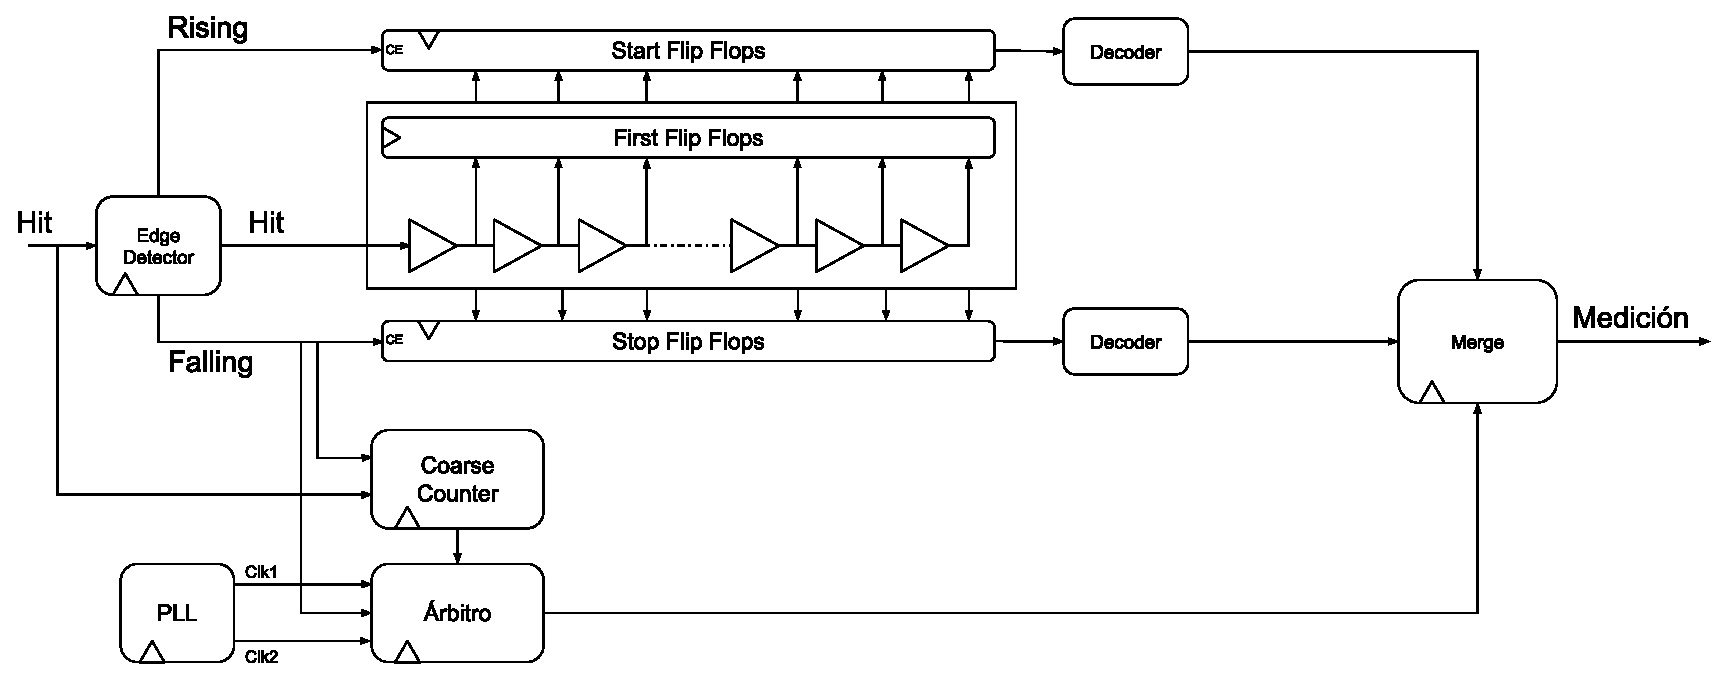
\includegraphics[width=0.75\textwidth]{imagenes/arq_tdc.eps}
     \caption{Arquitectura del TDC. Se ignora el routeo del clock.}
     \label{fig: TDC}
\end{figure}